\section{Práctica 1}

\subsection{}

\subsubsection{}
$I(s) = -log_2(P(s))$

\begin{tabular}{rl}
$H(S)$ & $= \sum_{s \in S}(P(s) I(s))$ \\
& $= (P(s_0) I(s_0)) + (P(s_1) I(s_1))$ \\
& $= (p_0 (-log_2(p_0))) + (1 - p_0) (-log_2(1 - p_0)))$ \\
& $= -p_0 log_2(p_0) - log_2(1 - p_0) + p_0 log_2(1 - p_0)$ \\
& $= p_0(log_2(1 - p_0) -log_2(p_0)) - log_2(1 - p_0)$ \\
& $= p_0 * log_2(\frac{1 - p_0}{p_0}) - log_2(1 - p_0)$ \\
\end{tabular}

\subsubsection{}

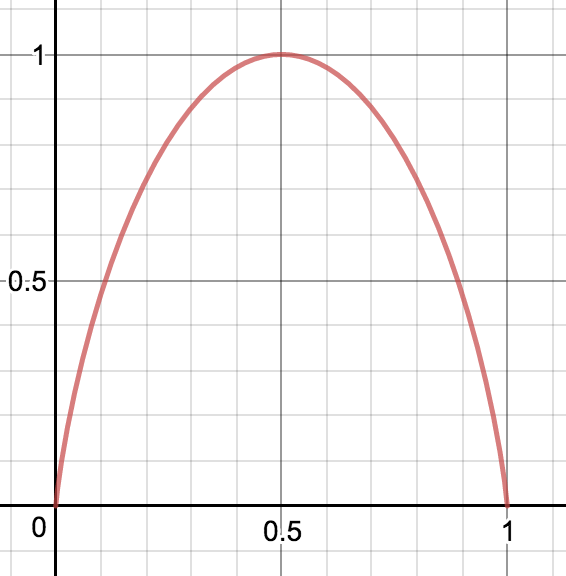
\includegraphics{imagenes/1_1_b.png}

\subsection{}

\subsubsection{}
El tercero

\subsubsection{}
El segundo y el tercero

\subsubsection{}
\begin{tabular}{rl}
$H(S)$ & $= \sum_{s \in S}(P(s) I(s))$ \\
& $= 0.4 (-log_2(0.4)) + 0.3 (-log_2(0.3)) + 0.2 (-log_2(0.2)) + 0.1 (-log_2(0.1))$ \\
& $= 1.84643934467$ \\
\end{tabular}

\begin{tabular}{rl}
$L(segundo)$ & $= \sum_{s \in S}(P(s)|C(s)|)$ \\
& $= 0.4 * 1 + 0.3 * 2 + 0.2 * 3 + 0.1 * 3$ \\
& $= 1.9$ \\
\end{tabular}

\begin{tabular}{rl}
$L(tercero)$ & $= \sum_{s \in S}(P(s)|C(s)|)$ \\
& $= 0.4 * 1 + 0.3 * 2 + 0.2 * 3 + 0.1 * 4$ \\
& $= 2$ \\
\end{tabular}

Eficiencia segundo: 0,9718101814

Eficiencia tercero: 0,9232196723

El segundo es más eficiente.

\subsubsection{}
No, puesto que $H(S) \leq L(C)$ en ambos casos.

\subsection{}

\subsubsection{}
\begin{tabular}{rl}
$H(S)$ & $= \sum_{s \in S}(P(s) I(s))$ \\
& $= 0.5 (-log_2(0.5)) + 0.5 (-log_2(0.5))$ \\
& $= 1$ \\
\end{tabular}

\begin{tabular}{rl}
$L(C)$ & $= \sum_{s \in S}(P(s) |C(s)|)$ \\
& $= 0.5 * 1 + 0.5 * 1$ \\
& $= 1$ \\
\end{tabular}

\subsubsection{}
\begin{tabular}{rl}
$H(S)$ & $= \sum_{s \in S}(P(s) I(s))$ \\
& $= 0.25 (-log_2(0.25)) + 0.25 (-log_2(0.25)) + 0.25 (-log_2(0.25)) + 0.25 (-log_2(0.25))$ \\
& $= 2$ \\
\end{tabular}

\begin{tabular}{rl}
$L(C)$ & $= \sum_{s \in S}(P(s) |C(s)|)$ \\
& $= 0.25 * 2 + 0.25 * 2 + 0.25 * 2 + 0.25 * 2$ \\
& $= 2$ \\
\end{tabular}

\subsubsection{}
\begin{tabular}{rl}
$H(S)$ & $= \sum_{s \in S}(P(s) I(s))$ \\
& $= \frac{1}{6} (-log_2(\frac{1}{6})) + \frac{1}{6} (-log_2(\frac{1}{6})) + \frac{1}{6} (-log_2(\frac{1}{6})) + \frac{1}{6} (-log_2(\frac{1}{6})) + \frac{1}{6} (-log_2(\frac{1}{6})) + \frac{1}{6} (-log_2(\frac{1}{6}))$ \\
& $= 2.58496250072$ \\
\end{tabular}

\begin{tabular}{rl}
$L(C)$ & $= \sum_{s \in S}(P(s) |C(s)|)$ \\
& $= \frac{1}{6} (-log_2(\frac{1}{6})) + \frac{1}{6} (-log_2(\frac{1}{6})) + \frac{1}{6} (-log_2(\frac{1}{6})) + \frac{1}{6} (-log_2(\frac{1}{6})) + \frac{1}{6} (-log_2(\frac{1}{6})) + \frac{1}{6} (-log_2(\frac{1}{6}))$ \\
& $= 2.58496250072$ \\
\end{tabular}

\subsubsection{}
\begin{tabular}{rl}
$H(S)$ & $= \sum_{s \in S}(P(s) I(s))$ \\
& $= 0.125 (-log_2(0.125)) * 8$ \\
& $= 3$ \\
\end{tabular}

\subsubsection{}
\begin{tabular}{rl}
$H(S)$ & $= \sum_{s \in S}(P(s) I(s))$ \\
& $= 0.1 (-log_2(0.1)) * 10$ \\
& $= -log_2(0.1)$ \\
& $= log_2(10)$ \\
& $= 3.32192809489$ \\
\end{tabular}

\subsubsection{}
\begin{tabular}{rl}
$H(S)$ & $= \sum_{s \in S}(P(s) I(s))$ \\
& $= \frac{1}{n} (-log_2(\frac{1}{n})) * n$ \\
& $= -log_2(\frac{1}{n})$ \\
& $= log_2(n)$ \\
\end{tabular}

\subsection{}
Acá lo mas importante es notar que cada vez que la fuente $D$ toma un símbolo
es independiente de la anterior, entonces se puede definir
$P_D(s) = (P_D(A) * P_A(s) si s \in A sino P_D(B) * P_B(s))$, con $P_D(A)$ y
$P_D(B)$ la probabilidad de que $D$ saque un símbolo de $A$ y de $B$,
respectivamente. Entonces la solución sería:

\begin{enumerate}
\item $P_D(s) = 1/16$ si $s \in A$ sino $1/32$, no es equiprobable
\item $P_D(s) = 1/64$ si $s \in A$ sino $3/64$, no es equiprobable
\item $P_D(s) = 1/32$ si $s \in A$ sino $3/64$, no es equiprobable
\item $P_D(s) = 1/12$ si $s \in A$ sino $1/48$, no es equiprobable
\end{enumerate}

\subsection{}

\subsubsection{}
Como la fuente es equiprobable:

\begin{tabular}{rl}
$H(S) $ & $= log_2|S|$ \\
&$= log_2(10^{640*480})$ \\
&$= 640 * 480 * log_2(10)$ \\
\end{tabular}

\subsubsection{}
En esta fuente equiprobable, tenemos que $H(S) = log_2(n)$, no siendo $n$ una potencia de 2. Esto implica que no podemos pensar en recurrir a un código (óptimo) que asigne $log_2(n)$ bits por imagen, pues por supuesto estos valores deben ser números enteros. No obstante, la aproximación más cercana a este valor es tomar exactamente $\lceil log_2(n) \rceil$ bits por imagen. De esta forma podremos armar un código que sea unívocamente decodificable (cada imagen recibe una tira de bits distinta) y localmente óptimo, entendiendo por esto que todo otro código que mapee cada imagen a una tira de bits de igual largo debe necesariamente poseer una longitud media igual o mayor.
Como nota adicional, extrapolando los conceptos plasmados en la resolución de este ejercicio, es interesante pensar en si, efectivamente, dada una fuente equiprobable S' de m símbolos, y dado un código C que actúe sobre S' definiendo para cada símbolo una codificación de largo $\lceil log_2(m) \rceil$ bits, se tiene que C es óptimo. Cuando m es potencia de 2, la respuesta es afirmativa (¿por qué?). En cualquier otro caso, y quizás yendo a contramano de la intuición, la respuesta es que no. Como ejemplo sencillo, considerar el caso en el que $m = 3$. Como $\lceil log_2(m) \rceil = 2$, tenemos que $L(C) = 2$. Sin embargo, podemos proponer un código alternativo C' que asigne un 0 a un símbolo, un 10 a otro y un 11 al restante. Es claro que C' es instantáneo, y además se ve claramente que $L(C') < 2 = L(C)$

\subsubsection{}
Para responder este ítem, hay que usar el teorema de Shannon: $C = B * log_2(1 + SNR)$. Primero, la relación señal-ruido hay que pasarla de decibeles a veces: $SNR = 10^{30/10} = 1000$. Luego, como se necesitan 30 imágenes por segundo, la capacidad de canal debe ser mayor o igual que $\lceil 640 * 480 * log_2(10) * 30 \rceil$ bps. Entonces, $B = (\lceil 640 * 480 * log_2(10) \rceil * 30)/ log_2(1001)$ Hz.

\subsection{}
Para calcular la capacidad de volumen, necesitamos $Delay$ y $V_{tx}$. Primero calculamos la Capacidad de Transmisión de Shannon para obtener la $V_{tx}$ (dejamos la resolución para el inciso b):

\begin{tabular}{rl}
$C$ & $= B * log_2(1 + SNR[dB])$ \\
& $= 400kHz * log_2(1 + 10[dB])$ \\
& $= 400kHz * log_2(1 + 10[veces]) \implies V_{tx} \leq 1383,7Kbps$ \\
\end{tabular}

Ahora Delay:

\begin{tabular}{rl}
$Delay$ & $= T_{prop} + T_{tx}$ \\
& $= \frac{D}{V_{prop}} + \frac{|Unidad de Datos|}{V_{tx}}$ \\
& $= \frac{100km}{200000km/s} + \frac{1bit}{1383Kbps} = 0,0005seg = 0,5ms$ \\
\end{tabular}

Finalmente:

$C_{vol} = Delay * V_{tx} = 691bits$

\subsection{}
$C_{max} = 100$Mbps \\
$V_{prop} = 300000$ km/s \\

\begin{tabular}{rl}
$Delay$ & $= T_{tx} + T_{prop}$ \\
$Delay$ & $= \frac{|datos|}{V_{tx}} + \frac{D}{V_{prop}}$ \\
$Delay$ & $= \frac{30Mb}{100Mbps} + \frac{D}{300000km/s}$ \\
$0.04s$ & $\geq \frac{30Mb}{100Mbps} + \frac{D}{300000km/s}$ \\
$0.04s - \frac{30Mb}{100Mbps}$ & $\geq \frac{D}{300000km/s}$ \\
$0.04s - 0.3$s & $\geq \frac{D}{300000km/s}$ \\
$(- 0.26)s * 300000km/s$ & $\geq D$ \\
$-78000km/s$ & $\geq D$ \\
\end{tabular}

No pueden existir distancias negativas. Siendo la velocidad de transmicion de 100 Mpbs, no pueden enviarse 30 Mb en menos de 0.3 s.

\subsection{}
\subsubsection{}
\begin{tabular}{rl}
$Delay$ & $= T_{prop} + T_{tx}$ \\
& $= \frac{D}{V_{prop}} + \frac{|Unidad de Datos|}{V_{tx}}$ \\
& $= \frac{385000km}{300000km/s} + \frac{1bit}{100Mbps}$ \\
& $= 1.29s$
\end{tabular}

$RTT = Delay * 2 = 2.58s$

\subsubsection{}
\begin{tabular}{rl}
$C_{vol}$ & $= Delay * V_{tx}$ \\
& $= 2.58s * 100Mbps$ \\
& $= 258Mb$ \\
\end{tabular}

\subsubsection{}
\begin{tabular}{rl}
$T_{total}$ & $= Delay_{ida} + Delay_{vuelta}$ \\
& $= T_{prop} + T_{tx_{ida}} + T_{prop} + T_{tx_{vuelta}}$ \\
& $= \frac{D}{V_{prop}} + \frac{|Unidad de Datos|_ida}{V_{tx}} + \frac{D}{V_{prop}} + \frac{|Unidad de Datos|_vuelta}{V_{tx}}$ \\
& $= \frac{2D}{V_{prop}} + \frac{|Unidad de Datos|_ida + |Unidad de Datos|_vuelta}{V_{tx}}$ \\
& $= \frac{2 * 385000km}{300000km/s} + \frac{2Kb + 25Mb}{100Mbps}$ \\
& $= 2.57s + \frac{2Kb + 25000Kb}{100000Kbps}$ \\
& $= 2.57s + \frac{25002Kb}{100000Kbps}$ \\
& $= 2.57s + 0.25s$ \\
& $= 2.82s$ \\
\end{tabular}
